
\par{Listing \ref{private_local_memory_kernel} shows the kernel that uses together \emph{private memory} to bring elements of A to 
    on-chip memory and \emph{local memory} to cache column B. In 
    this case the amount of \emph{local memory} to use is passed to the kernel as the fourth argument. The main idea for this is
    that all work items share the same column of B to avoid going into \emph{global memory}.}

\par{As in the previous kernel line \emph{12} shows the copy of elements to \emph{private memory} and line \emph{15} shows the 
    copy of elements from \emph{global memory} to \emph{local memory}, also ...\emph{expand on the use of barriers}.}

\lstinputlisting[float,caption={Kernel making use of \emph{private memory} and \emph{local memory}.},label={private_local_memory_kernel}, 
                style=customc]{/Users/clalanne/GitHubProjects/OpenCLNotes/src/code/private_local_memory.c}

\par{Figure \ref{RowsCols} shows the results of this kernel for different architectures, not all \emph{work group} dimensions 
    were possible to execute for this \emph{kernel}. For the case of the Xeon and Xeon Phi from the 32x32 the runtime returned
    error -5, that means was a failure to allocate resources\cite{opencl_error}, this mainly is because we are forcing to the 
    allocation of local memory ~16KB per \emph{work item}.

\begin{figure}[!h]
    \centering
    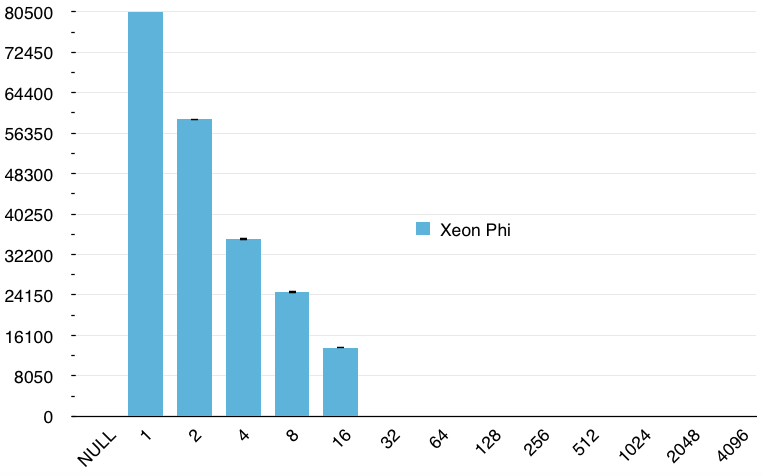
\includegraphics[width=0.49\textwidth]{figures/opt3_phi.png}
    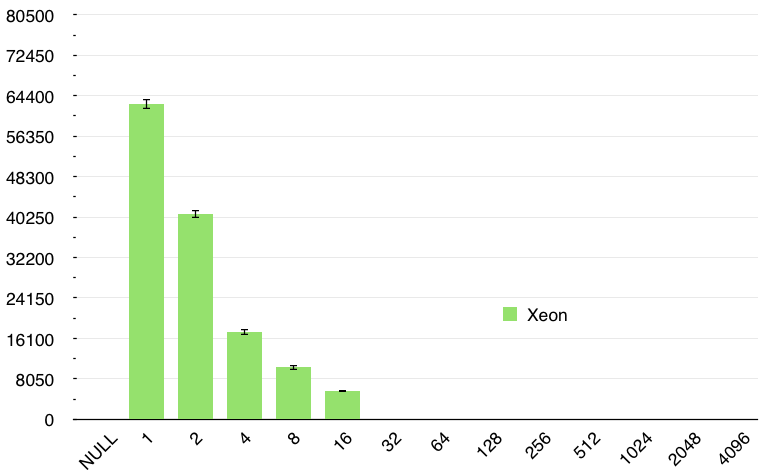
\includegraphics[width=0.49\textwidth]{figures/opt3_cpu.png}
    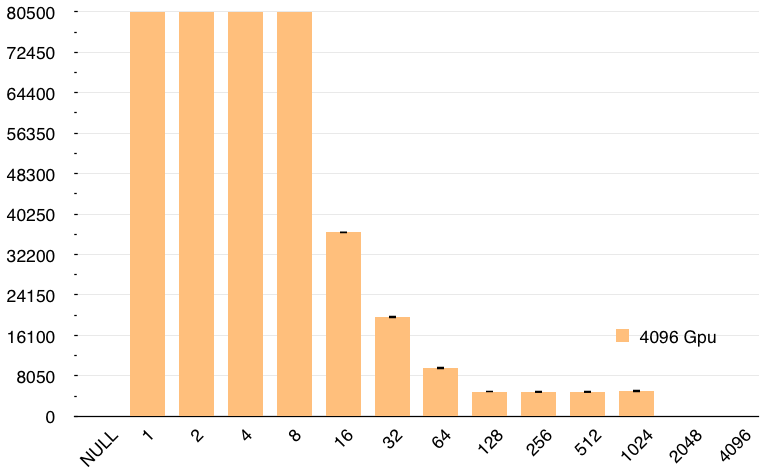
\includegraphics[width=0.49\textwidth]{figures/opt3_gpu.png}
    \caption{Rows and columns optimisation matrix multiplication in different architectures.}
    \label{RowsCols}
\end{figure}

\par{It seems to be a trade off here, between the the loop necesary to execute the copy of elements of B to \emph{local memory}
    (expensive gathering operations with a very poor L1 hit ratio) and the performance achieve in the loop where the kernel executes
    the computation(\emph{maybe vtune shot}).}

\par{In this case the best time is achived again by the GPU as we can see in figure \ref{RowsColsComp}, Also we can notice that the only 
    architectures that is able to take advantage of this optimisation is the Xeon. The Xeon Phi even have a warning in its 
    documentation about not using \emph{local} memory explicitelly as in this case, because of the cache system already is using 
    automatically this memory, and even warn about possible overhead time if this memory is defined explicitely\cite{opencl_phi}.}

\begin{figure}[!h]
    \centering
    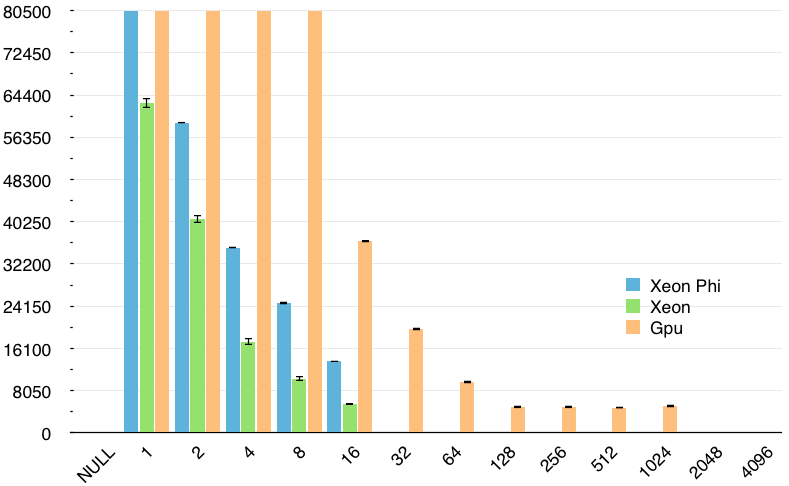
\includegraphics[width=0.6\textwidth]{figures/opt3_comp.png}
    \caption{Rows and columns optimisation matrix multiplication with more work in different architectures comparison.}
    \label{RowsColsComp}
\end{figure}

